\documentclass[12pt]{amsart}

%%%%%%%%%%%%%%%%%%%%%%
%----- PREAMBLE -----%
%%%%%%%%%%%%%%%%%%%%%%

%----- ENCODINGS -----%

\usepackage[utf8]{inputenc}
\usepackage[T1]{fontenc}

%----- TYPOGRAPHY -----%

\usepackage[english]{babel}

%----- MATH SYMBOLS -----%

\usepackage{amsmath}
\usepackage{amssymb}
\usepackage{amsthm}

\usepackage{dsfont}
\usepackage{mathrsfs}
\usepackage{stmaryrd}

\usepackage{colonequals}

%--- Trucs retirés ----%

% \usepackage{latexsym}
% \usepackage{changepage}
% \usepackage{bbm}

%----- COLORS -----%

\usepackage{xcolor}
\definecolor{forestgreen}{rgb}{0.27, 0.60, 0.46} 

%----- FIGURES -----%

\usepackage{mdframed}

\usepackage{graphicx}

\usepackage{caption}

\usepackage{tikz}
\usetikzlibrary{arrows}
\usetikzlibrary{decorations.markings}
\usepackage{tikz-cd}
\usetikzlibrary{fpu}

\usepackage{pgf}
\usepackage{pgfplots}
\pgfplotsset{compat=1.15}

\usepackage{forest}

\forestset{
  Bseries/.style={
    for tree={
      grow'=90,
      parent anchor=center,
      child anchor=south,
      minimum width=1pt,
      inner sep=1pt,
      s sep=3pt,
      circle,
      if level=0{
        baseline
      }{},
      l = 3pt,
      if n children=0{tier=terminal}{}
    },
    %before computing xy={
    %  for tree={
    %    l= 12pt,
    %  }
    %}
  }
}
\newcommand\Bseries[1]{\Forest{Bseries #1}}

\forestset{
  Cseries/.style={
    for tree={
      grow'=90,
      parent anchor=center,
      child anchor=center,
      minimum width=1pt,
      inner sep=0pt,
      s sep=2.5pt,
      circle,
      if level=0{
        baseline
      }{}
    },
    before computing xy={
      for tree={
        l=5pt,
      }
    }
  }
}
\newcommand\Cseries[1]{\Forest{Cseries #1}}
% \usepackage[inkscapelatex=false]{svg}

%----- PAGE LAYOUT -----%

\oddsidemargin  =5mm
\evensidemargin =5mm
\topmargin      =5mm
\textwidth      =150mm
\textheight     =200mm

\usepackage{changepage}

\usepackage{fancyhdr}
\pagestyle{fancy}
\fancyhead[L]{} % remove title from the header
\fancyhead[R]{\thepage} % add page number on top right
\renewcommand{\headrulewidth}{0pt} % removes horizontal mine
\fancyfoot{} % empty the footer

%----- BIBLIOGRAPHY -----%

\usepackage[backend=biber,style=numeric]{biblatex}
\addbibresource{Biblio.bib}

%----- REVISIONS -----%

\usepackage{todonotes}

%----- LABELS -----%

% \usepackage{upref}

%----- HYPER LINKS -----%

\usepackage{hyperref}
\hypersetup{
 colorlinks,
 linkcolor={red!50!black},
 citecolor={blue!50!black},
 urlcolor={blue!80!black}
}

%----- THEOREM ENVS -----%

\theoremstyle{plain}
\newtheorem{teo}{Theorem}[section]
\newtheorem{prop}[teo]{Proposition}
\newtheorem{cor}[teo]{Corollary}
\newtheorem{lem}[teo]{Lemma}
\newtheorem{conj}[teo]{Conjecture}

\theoremstyle{definition}
\newtheorem{defi}[teo]{Definition}

\theoremstyle{remark}
\newtheorem{rema}[teo]{Remark}
\newtheorem{remas}[teo]{Remarks}
\newtheorem{exemple}[teo]{Example}
\newtheorem{exemples}[teo]{Examples}
\newtheorem{constr}[teo]{Construction}
\newtheorem{por}[teo]{Porism}
\newtheorem{notat}[teo]{Notation}

%----- MACROS -----%

\DeclareMathOperator{\Hom}{Hom}
\DeclareMathOperator{\Mon}{Mon}
\DeclareMathOperator{\Op}{Op}
\DeclareMathOperator{\End}{End}
\DeclareMathOperator{\SymMon}{SymMon}
\DeclareMathOperator{\Fun}{Fun}
\DeclareMathOperator{\hocolim}{hocolim}
\DeclareMathOperator{\colim}{colim}
\DeclareMathOperator{\sSet}{sSet}
\DeclareMathOperator{\emb}{emb}
\DeclareMathOperator{\card}{card}
\DeclareMathOperator{\Sing}{Sing}
\DeclareMathOperator{\Diffeo}{Diffeo}
\DeclareMathOperator{\Moore}{Moore}
\DeclareMathOperator{\Conf}{Conf}
\DeclareMathOperator{\UConf}{UConf}
\DeclareMathOperator{\id}{id}
\DeclareMathOperator{\triv}{triv}
\DeclareMathOperator{\Top}{Top}
\DeclareMathOperator{\Diag}{Diag}
\DeclareMathOperator{\Pos}{Pos}
\DeclareMathOperator{\disc}{disc}
\DeclareMathOperator{\HT}{HT}
\DeclareMathOperator{\BT}{BT}
\DeclareMathOperator{\Ob}{Ob}
\DeclareMathOperator{\Mor}{Mor}
\DeclareMathOperator{\Id}{Id}
\DeclareMathOperator{\standard}{standard}
\DeclareMathOperator{\Spaces}{Spaces}
\DeclareMathOperator{\Map}{Map}
\DeclareMathOperator{\im}{im}
\DeclareMathOperator{\ext}{ext}
\DeclareMathOperator{\Max}{max}
\DeclareMathOperator{\Aut}{Aut}
\DeclareMathOperator{\Cof}{Cof}
\DeclareMathOperator{\splitt}{split}
\DeclareMathOperator{\glue}{glue}
\DeclareMathOperator{\double}{double}
\DeclareMathOperator{\pc}{pc}

\newcommand{\Holink}{\mathcal{H}o\mathrm{Link}}
\newcommand{\iso}{\overset{\sim}{=}}
\newcommand{\op}{\mathcal{O}}
\newcommand{\C}{\mathcal{C}}
\newcommand{\s}{\mathcal{S}}
\newcommand{\E}{\mathcal{E}}
\newcommand{\F}{\mathcal{F}}
\newcommand{\V}{\mathcal{V}}
\newcommand{\W}{\mathcal{W}}
\newcommand{\Y}{\mathcal{Y}}
\newcommand{\T}{\mathcal{T}}
\newcommand{\G}{\mathcal{G}}

\newcommand\mlnode[1]{\begin{tabular}{@{}c@{}}#1\end{tabular}}

%%%%%%%%%%%%%%%%%%%%%%
%----- DOCUMENT -----%
%%%%%%%%%%%%%%%%%%%%%%

\title{Trees and their degrees}
\author{Marie-Camille Delarue}
\date{\today}

\begin{document}

\maketitle
\tableofcontents

\section{Introduction}

In the course of my study of the family of Higman--Thompson groups, 
there arose a question that was easy to answer in small dimensions
and much harder in higher dimensions.
The fundamental reason for this is that it was easy to come up with a reasonable visualization in low dimensions,
and much harder in higher dimensions because of the limitations of 3-dimensional space.
Therefore, we tried to come up with a good visualization in higher dimensions.

The following document explains this problem and the framework we came up with to answer it in higher dimensions.
Reading the following document is recommended to understand the specific question we were working on as well as its implementation.

\section{A question about trees}\label{treeprob}

Topological spaces are easier to understand when broken up into building blocks, which are simple spaces, and maps between them.
Let us say we have a space of trees. 
We break it up by understanding all the individual junctions, and how the junctions attach to each other.
We will consider finite rooted trees, and we call an \textbf{$a$-junction} a vertex of the tree with one parent and $a$ children: 
For instance, \Cseries{[[[][][]]]} is a 3-junction.
Let us first consider the case of trees with simple junctions.

\subsection{Trees with simple junctions}
Consider a finite rooted tree which only has $a$-junctions, for $a$ an integer.
We will think of trees as being oriented from the leaves to the root.
The following is an illustration of an (oriented) junction:
\begin{center}
  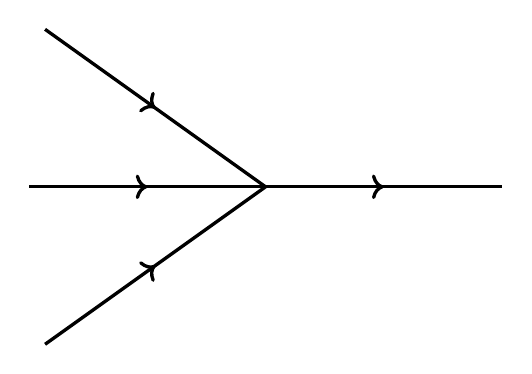
\begin{tikzpicture}
\begin{scope}[very thick,decoration={
  markings,
  mark=at position 0.5 with {\arrow{>}}}
  ] 
  \draw[postaction={decorate}] (-2.8,2)--(0,0);
  \draw[postaction={decorate}] (-3,0)--(0,0);
  \draw[postaction={decorate}] (-2.8,-2)--(0,0);
  \draw[postaction={decorate}] (0,0)--(3,0);
\end{scope}
  \end{tikzpicture}
\end{center}
We will call \textbf{degree} of a junction the number of incoming edges minus the number of outgoing edges at the junction.
For any $a$-junction, this number is clearly $a-1$.
If the trees have two or more types of junctions, for instance $a$-junctions and $b$-junctions,
the $a$-junctions have degree $a-1$, and the $b$-junctions have degree $b-1$.

\subsection{Trees with double junctions}

Now let us consider a family of trees with both $a$-junctions and $b$-junctions, for $a$ and $b$ two different integers, 
with the following additional \textbf{interchange relation}:
\begin{center}
  \Bseries{[[, edge = orange,[, edge = purple][, edge = purple]][, edge = orange,[, edge = purple][, edge = purple]][,edge = orange,[, edge = purple][, edge = purple]]]} = \Bseries{[[, edge = purple,[, edge = orange][, edge = orange][, edge = orange]][, edge = purple,[, edge = orange][, edge = orange][, edge = orange]]]}.
\end{center} 
This means that we identify certain trees even if they do not have the same shape.
How can we represent this equality topologically?
In topology, we can always relax an equality between two objects by creating a path between them.
We add an $ab$-junction which represents this path:
\begin{center}
  \Bseries{[,phantom,s sep = 5pt,[[, edge = forestgreen][, edge = forestgreen][, edge = forestgreen][, edge = forestgreen][, edge = forestgreen][, edge = forestgreen]]
  [[, edge = orange,label = {[label distance=0cm]180:$\rightarrow$}[, edge = purple][, edge = purple]][, edge = orange,[, edge = purple][, edge = purple]][,edge = orange,[, edge = purple][, edge = purple]]]]}
  
  
   \Bseries{[,phantom,s sep = 5pt, [[, edge = forestgreen][, edge = forestgreen][, edge = forestgreen][, edge = forestgreen][, edge = forestgreen][, edge = forestgreen]]
   [[, edge = purple,label = {[label distance=0.05cm]180:$\rightarrow$}[, edge = orange][, edge = orange][, edge = orange]][, edge = purple,[, edge = orange][, edge = orange][, edge = orange]]]]}
  \end{center}

If our tree lives in $N$-dimensional space, we are adding an extra dimension which represents time.
The position of $t$ in $[0,1]$ indicates what the form of the tree is in a continuous way as depicted in figure \ref{timeline}.
Now our tree is parametrized by an element in $[0,1]^{N+1}$.
\begin{figure}
  \def\svgwidth{0.8\hsize}
  \input{timeline.pdf_tex}
  \caption{The tree is parametrized by $(x,t)\in[0,1]^N\times [0,1]$. 
  The barycenter of the junctions is governed by $x$ and the shape of the tree (including how far apart the junctions are) is governed by $t$.}
  \label{timeline}  
\end{figure}
  
\begin{mdframed}[backgroundcolor=purple!10]
In the program, there is a function \texttt{make\char`_family} which holds the combinatorial information about the tree,
and a function \texttt{tree\char`_at} which to a point in $[0,1]^{N+1}$ and the combinatorial information of the tree
associates the corresponding embedding of a tree inside a unit cube $[0,1]^N$.
\end{mdframed}

\subsection{Goal -- notion of degree}
We would like to determine the degree of this extra junction. 
It is tempting to say that the degree of this junction is $ab-1$.
However, we now have equivalent trees that do not have the same structure, so how can one determine the degree in this case?

Let's give another definition of the degree by going back to the case of a simple junction.
We represent the junction living inside a small neighborhood, depicted as a circle around it in figure \ref{simple}.
Then imagine a smaller lens traveling around the boundary of the small neighborhood and recording what it sees.
The lens will see a single path $a+1$ times:
$a$ time with positive orientation and once with negative orientation, and so we recover a total degree of $a-1$.
\begin{figure}
\begin{center}
  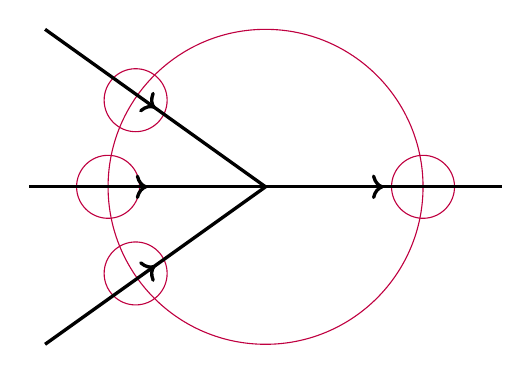
\begin{tikzpicture}
    \draw[draw = purple] (0,0) circle (2cm);
    % Tiny circles on boundary
    \draw[draw = purple] (-1.65,1.1) circle (0.4cm);
    \draw[draw = purple] (-2,0) circle (0.4cm);
    \draw[draw = purple] (2,0) circle (0.4cm);
    \draw[draw = purple] (-1.65,-1.1) circle (0.4cm);

\begin{scope}[very thick,decoration={
  markings,
  mark=at position 0.5 with {\arrow{>}}}
  ] 
  \draw[postaction={decorate}] (-2.8,2)--(0,0);
  \draw[postaction={decorate}] (-3,0)--(0,0);
  \draw[postaction={decorate}] (-2.8,-2)--(0,0);
  \draw[postaction={decorate}] (0,0)--(3,0);
\end{scope}
  \end{tikzpicture}
\end{center}
\caption{The case of a simple junction}
\label{simplej}
\end{figure}

We will find the degree of the $ab$-junction by traveling around it and recording what we see.
We need to count the number of $a$-junctions and $b$-junctions that we see around it.
This is how we will construct the detector map.

\section{Defining the detector map}
We create a detector for $a$-junctions, and one for $b$-junctions,
according to the following procedure.
Given a specific embedding of a tree inside a cube,
we look at a smaller detector cube centered inside the unit cube and we record what it contains:
\begin{itemize}
\item if it contains a single $a$-junction and no other connected component of the tree, 
we record the position of the $a$-junction, which is a point inside the detector cube,
and rescale it to a point of the unit cube.
\item if it contains anything else, we record "nothing", which we set as the basepoint.
\end{itemize}
Therefore, the range of the detector map is a unit cube $[0,1]^N$, whose boundary has been collapsed to a point,
which we call the basepoint. 

\begin{mdframed}[backgroundcolor=purple!10]
  \centering 
  The detector map that we define in the program is actually a composition of \texttt{tree\char`_at} and the aforementioned procedure:\\
\begin{itemize}
\item Take a point in the cube $[0,1]^{N+1}$ that we can write $(x,t)$ where $x\in[0,1]^N, t\in[0,1]$;
\item Construct an embedding of a tree inside the cube $[0,1]^N$. The barycenter of the junctions is at $x$ and the shape of the tree is determined by $t$;
\item Look inside a smaller detector cube and record what you see;
\item Get a point in $([0,1]^N)/(\partial [0,1]^N)$.
\end{itemize}
This is what the functions \texttt{detect\char`_a} and \texttt{detect\char`_b} correspond to.
\end{mdframed}

\section{Degree of a map between spheres}
The detector map is defined from $[0,1]^{N+1}$ to $[0,1]^N/\partial [0,1]^N$.
If we restrict the source to the boundary of $[0,1]^{N+1}$, then the source is equivalent to an $N$-sphere.
The range $[0,1]^N/\partial [0,1]^N$ is a cube whose boundary is collapsed to a point, 
which is also equivalent to an $N$-sphere, as illustrated in figure \ref{sphere}.
\begin{figure}
  \def\svgwidth{0.4\hsize}
  \input{spheresandcubes.pdf_tex}
  \caption{The boundary of the 3-dimensional cube and a 2-square whose boundary is glued onto a point 
  are both models for the 2-sphere.}
  \label{sphere}
\end{figure}
Therefore, the detector map is equivalent to a function from a sphere $S^N$ to itself.

The notion of degree we defined in section \ref{treeprob} is closely related 
to the notion of degree of maps between spheres.
Basically, the degree of a map from a sphere $S^N$ to itself is the number of times 
the map goes around the target sphere, up to homotopy.
It is clearer to see this on an example.
\begin{exemple}
  Imagine the function from the circle $S^1$ to another $S^1$ which wraps the circle around itself twice,
  as illustrated in figure \ref{degre2}:
  \begin{figure}
    \def\svgwidth{0.4\hsize}
    \input{degre2.pdf_tex}
    \caption{The orange circle wraps twice around the first one, starting and ending at the purple point.}
    \label{degre2}
  \end{figure}
  The degree of this map is $2$.
\end{exemple}
Examples on spheres of higher dimension are more difficult to understand than in dimension 1, but they work in the same way.

\subsection{Degree formula}
If the map is $C^1$, we can obtain the degree by picking a regular point $y$ in the image (i.e. a point with nonsingular differential),
and counting its preimages:
\[d = \displaystyle \sum_{p\in f^{—1}(y)} s_p\] 
where $s_p$ is the sign of the Jacobian of $f$ at point $p$.
\begin{exemple}
  Consider the two maps from $S^1$ to $S^1$ depicted in figure \ref{queldegre}:
  \begin{figure}
    \def\svgwidth{0.7\hsize}
    \input{queldegre.pdf_tex}
    \caption{The left map is the one introduced earlier.
    The map on the right wraps the orange circle around the black circle once, then changes directions and wraps around it once more.}
    \label{queldegre} 
  \end{figure}
    If one were simply to count the preimages at any regular value -- for instance, not at the basepoint of the circle (the purple point),
    one would see that for both maps, there are two points of the orange circle mapped to the same point of the black circle.
    However, the degree of the left map is 2, and the degree of the right map is 0.
    This is because in the first instance, both preimages contribute the same sign to the formula: they are oriented in the same way.
    In the second instance, they have opposite orientation.
\end{exemple}

\subsection{Algorithm}
Let us now go through the steps of the algorithm:
\begin{enumerate}
\item Pick a regular value $y$ (more on this in the next section).
\item Discretize the domain $[0,1]^N$ with a regular grid.
\item Scan each cell to identify those which are likely to contain a preimage of $y$.
\item Perform a Newton iteration on the retained cells to get an approximate preimage of $y$
\item Compute the Jacobian at the preimage and get the sign of its determinant.
\item Add up the signs of all found preimages.
\end{enumerate}

Because Newton's method is a bit expensive, we want to have a good test to determine if a cell is likely to contain a preimage of $y$.
We perform a bounding box testin step 3: for the cell $C$ with set of corners $V$, 
we consider the box $\displaystyle \prod[\min_{x\in V}f(x)_i,\max_{x\in V}f(x)_i].$
If $y$ is not in this box, we discard the cell as unlikely to contain a preimage of $y$.
This works when the detector map is reasonable.

\textbf{Picking a regular value for step 1:}
It is very important to pick a good regular value to carry out the above procedure.
For maps with a clear analytic formula, this is easy to determine.
For the detector map, this is not so clear. What we do is look at the outputs of the detector map,
and pick a regular value that lives inside a cluster of other regular values, to make sure it is in a very regular zone.

\section{Limitations}

\subsection{Limitations of the degree computation}
The most time-consuming process is definitely the degree computation, as its complexity is in $O(s^N\times N)$
where $s$ is the number of points in the grid.
When $N\geq 5$, only extremely simple computations work.
Some possible fixes include doing fewer Newton iterations or computing the Jacobian in a coarser way,
but the best idea would probably be to create a grid which is not uniform.
We could start with a coarse grid, and mark the cells which are likely to contain a preimage of our value,
only subdivide those cells with a finer grid, and repeat the process until we get a few candidate cells.

We could also use more sophisticated programs to find roots, such as.

\subsection{Other problems}
We also note that the model for trees is not that readily adaptable to trees with triple junctions,
i.e. the case of trees with $a$-junctions, $b$-junctions, and $c$-junctions,
which are allowed to collide and switch pairwise.

\end{document}
